\documentclass{article}

\author{Pedro Henrique Limeira da Cruz}
\title{Resistência dos Materiais - I}

\usepackage[margin=0.8in]{geometry}
\usepackage{indentfirst}
\usepackage{fancyhdr}
\usepackage{tcolorbox}
\usepackage{graphicx}
\usepackage{amsmath}
\usepackage{amssymb}
\usepackage{enumitem}
\usepackage{tabularx} % in the preamble


% Create a Todo list
\newlist{todolist}{itemize}{2}
\setlist[todolist]{label=$\square$}


% Create a new command to be used in the align environment in multiple line equations do only the last equation is numbered  
\newcommand{\n}{\nonumber \\ }
\makeatletter
\let\inserttitle\@title
\makeatother
% Set the style of the page 
\pagestyle{fancy}
\fancyhf{}
\rhead{Pedro Henrique L. da Cruz}
\lhead{\inserttitle}
\rfoot{Page \thepage}

\usepackage{hyperref}
\hypersetup{
    colorlinks=true,
    linkcolor=black,
    filecolor=magenta,
    urlcolor=cyan,
}

% Begin the Document 
\begin{document}

    \maketitle
    \thispagestyle{empty}

    % Add the image inside a figure in as the first page
    \begin{figure}[h]
        \begin{center}
            
\includegraphics[scale = 0.15]{/Users/pedrocruz/Documents/UNICAMP/ES101/ES101 - Robotic Arm/img/unicamp.png}
        \end{center}
    \end{figure}

    % Change to the Next page 
    \newpage
    \tableofcontents
    \newpage

    \section{Introdução e Definições}

        A matéria de resistência dos materiais que iremos estudar nada mais é do que a análise de mecânica estática, só que, dessa vez, para corpos que se deformam.
        Levando isso em consideração, teremos primeiro que revisar alguns conceitos importantes de estática, sendo eles, de modo geral:
        \begin{itemize}
            \item Modelos de Suporte e Vínculos
            \item Equilíbrio Estático : cargas simples, combinadas, carregamentos distribuídos, ...
        \end{itemize}

        \subsection{Modelos de Suporte e Vínculos}

            Como o nosso objetivo é modelar o sistema para aplicarmos os equacionamentos de estática (e mais para frente outros mais específicos de ResMat) precisamos, primeiro, ser capazes de
            identificar as forças que atuam sobre o corpo em análise. Por isso remos revisar as diferentes forças de reação que cada tipo de suporte gera em uma viga:

            \begin{table}[h]
                \begin{tabular}{|l|c|c|c|l|l|}\hline
                    \textbf{Nome} & \textbf{Exemplo} & \textbf{Representação} & \textbf{D.C.L} & \textbf{Descrição} & \textbf{Cometário} \\ \hline

                    Rolete & 

                        \begin{minipage}{.2\textwidth}
                            \centering
                            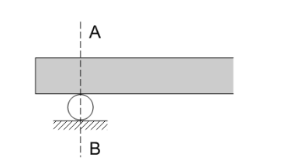
\includegraphics[width=\textwidth]{imgs/rolete_eg.png}
                        \end{minipage} &

                        \begin{minipage}{.2\columnwidth}
                            \centering
                            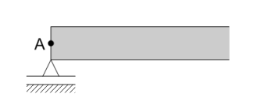
\includegraphics[width=\textwidth]{imgs/rolete_rep.png}
                        \end{minipage} &

                        \begin{minipage}{.2\columnwidth}
                            \centering
                            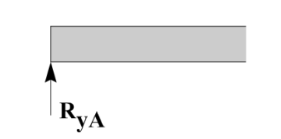
\includegraphics[width=.85\textwidth]{imgs/rolete_dcl.png}
                        \end{minipage} &

                        \begin{minipage}{.1\columnwidth}
                            \tiny
                            •Resistente a forças em \emph{somente uma linha de direção}

                                •Reação de apoio: 1 incógnita
                        \end{minipage}&

                        \begin{minipage}{.1\columnwidth}
                            \vspace{5px}
                            \tiny
                            Importante observar que a representação possui \textbf{DUAS} linhas horzontais abaixo do triângulo.
                            \vspace{5px}
                        \end{minipage} \\ \hline

                    Pino & 

                        \begin{minipage}{.2\textwidth}
                            \centering
                            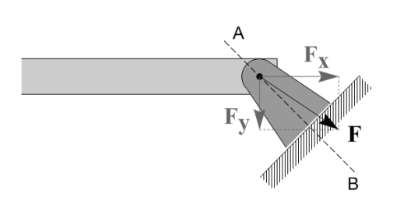
\includegraphics[width=\textwidth]{imgs/pino_eg.png}
                        \end{minipage} &

                        \begin{minipage}{.2\columnwidth}
                            \centering
                            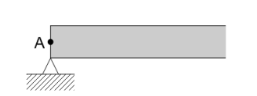
\includegraphics[width=\textwidth]{imgs/pino_rep.png}
                        \end{minipage} &

                        \begin{minipage}{.2\columnwidth}
                            \centering
                            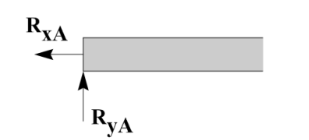
\includegraphics[width=\textwidth]{imgs/pino_dcl.png}
                        \end{minipage} &

                        \begin{minipage}{.1\columnwidth}
                            \tiny
                            •Resistente a forças em \emph{duas linhas de ação}

                            •Reação de apoio: 2 incógnitas
                        \end{minipage}&

                        \begin{minipage}{.1\columnwidth}
                            \vspace{5px}
                            \tiny
                            Importante observar que a representação possui somente \textbf{UMA} linha horzontai abaixo do triângulo.
                            \vspace{5px}
                        \end{minipage} \\ \hline


                        Engaste & 

                            \begin{minipage}{.2\textwidth}
                                \centering
                                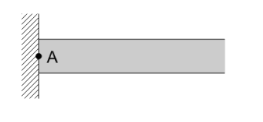
\includegraphics[width=\textwidth]{imgs/engaste_rep.png}
                            \end{minipage} &

                            \begin{minipage}{.2\columnwidth}
                                \centering
                                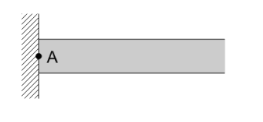
\includegraphics[width=\textwidth]{imgs/engaste_rep.png}
                            \end{minipage} &

                            \begin{minipage}{.2\columnwidth}
                                \centering
                                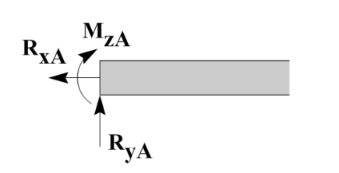
\includegraphics[width=\textwidth]{imgs/engaste_dcl.png}
                            \end{minipage} &

                            \begin{minipage}{.1\columnwidth}
                                \tiny
                                • Resiste a \textbf{Forças} e \textbf{Momentos}
                            \end{minipage}&

                            \begin{minipage}{.1\columnwidth}
                                \vspace{5px}
                                \tiny
                                Até o momento é o único vínculo que resiste a momento.
                                \vspace{5px}
                            \end{minipage} \\ \hline

                \end{tabular}
                \caption{Principais Suportes e Vínculos - 2D}
            \end{table}

            Tendo em vista que há diferentes suportes e vínculos, é importante entender o processo de escolha de vínculos durante análise de uma força/momento. Para tal, podemos nos perguntar:
            \begin{enumerate}
                \item \textbf{O apoio/vínculo impede algum movimento que será resultante da força sob análise?} Se a resposta for \emph{não}, podemos simplesmente desconsiderar o vinculo na nossa
                modelagem. Se a resposta for \emph{sim}, ele impede um movimento, podemos prosseguir para outras perguntas.
                \item \textbf{O apoio/vínculo impede que a peça "gire" como resultado da força?} Se a resposta for \emph{sim} isso significa que o suporte restringe tanto forças quanto
                \emph{momentos}. Como temos somente um vínculo (o engaste) que tem essa característica, podemos usa-lo durante nossa modelagem. Se a resposta for não, ficamos entre um rolete e um pino.
                \item \textbf{O apoio/vínculo impede a movimentação, que seria resultante da força, em mais de um eixo?} Se \emph{sim}, temos um pino. Caso contrário teremos um rolete.
            \end{enumerate}

        \subsection{Equilíbrio Estático}

            Como dito anteriormente, o ponto de partida de ResMat é a estática mecânica. Agora que já definimos os principais modelos de forças de reação, podemos descrever o equilíbrio estático
            (assim como foi feito durante o estudo de Estática).

            O principal conceito que rege o equilíbrio estático é que o sistema não possui aceleração, logo há a conservação tanto da quantidade de movimento linear quanto angular, resultando nas
            respectivas equações:

            $$\\$$

            \begin{minipage}{.5\linewidth}
                \begin{align*}
                    \sum \vec F = 0 \Rightarrow \begin{cases}
                        \sum F_x = 0 \\ 
                        \sum F_y = 0 \\ 
                        \sum F_z = 0
                    \end{cases} 
                \end{align*}
            \end{minipage}%
            \begin{minipage}{.5\textwidth}
                \begin{align*}
                    \sum \vec M = 0 \Rightarrow \begin{cases}
                        \sum M_x = 0 \\ 
                        \sum M_y = 0 \\
                        \sum M_z = 0
                    \end{cases}
                \end{align*}
            \end{minipage}


            $$\\$$

            Para problemas de sistemas planos, as equações se resumem à:

            $$\\$$

            \begin{minipage}{.5\textwidth}
                    \centering
                    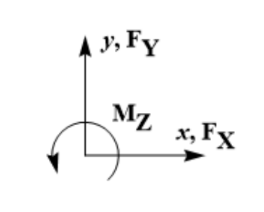
\includegraphics[width=.5\textwidth]{imgs/sis_plano.png}
            \end{minipage}%
            \begin{minipage}{.5\textwidth}
                \begin{align*}
                    \sum F_x = 0 \\ 
                    \sum F_y = 0 \\ 
                    \sum M_z = 0
                \end{align*}
            \end{minipage}

            A depender da topologia, no que tange equilíbrio estático, um sistema pode ser definido como:
            \begin{itemize}
                \item \textbf{Sistema Isostático}: As vinculações são suficientes para satisfazer o equilíbrio estático, número de incógnitas igual ao numero de equações.
                \item \textbf{Sistema Hiperestático}: As vinculações são em excesso para satisfazer o equilíbrio estático, número de incógnitas maior ao numero de equações.
                \item \textbf{Sistema Hipostático}: As vinculações não são suficientes para satisfazer o equilíbrio estático, número de incógnitas menor ao numero de equações.
            \end{itemize}

        \newpage
        \subsection{Carregamentos Combinados}
            Já vimos anteriormente no caso de cargas combinadas que, a depender das forças que o corpo sofre (e resiste) nós iremos representar os suportes e vínculos de uma forma específica. 
            Agora, nós iremos expandir esse assunto e descrever de forma detalhada os diferentes modelos que nós usamos para os corpos que sofrem essas forças e reações e descrever suas prioridades.

            A parte mais fundamental para entender o porque há diferentes modelos para descrever os corpos que \textbf{são esbeltos} (\emph{i.e} possuem comprimento muito maior que sua largura e
            altura) é:

            $$\\$$
            \begin{center}
                \textbf{Problemas de carregamento transversal, longitudinal e torsional são independentes}
            \end{center}
            $$\\$$

            Isso nos diz que podem haver problemas de carregamentos combinados que sejam necessários 3 modelos distintos para serem modelados, cada um com um modelo específico para o corpo, como
            podemos ver abaixo:

            \begin{table}[h]
                \centering
                \begin{tabular}{|l|c|l|c|}\hline
                    \textbf{Nome} & \textbf{Exemplo} & \textbf{Descrição} & \textbf{Equação} \\ \hline
                    Barra
                        &
                        \begin{minipage}{.4\textwidth}
                            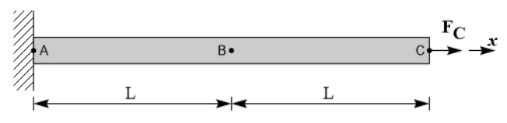
\includegraphics[width=\textwidth]{imgs/barra_eg.png}
                        \end{minipage}
                        &
                        \begin{minipage}{.3\textwidth}
                            Corpos sujeitos \textbf{somente a cargas logitudinais/axiais}
                        \end{minipage}
                        &
                        $\sum F_x = 0$ \\ \hline

                    Eixo 
                        &
                        \begin{minipage}{.4\textwidth}
                            \vspace{10px}
                            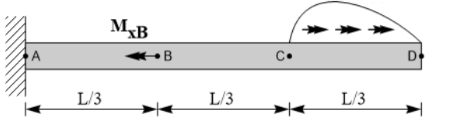
\includegraphics[width=.9\textwidth]{imgs/eixo_eg.png}
                        \end{minipage}
                        &
                        \begin{minipage}{.3\textwidth}
                            Corpos sujeitos \textbf{somente a cargas torcionais}
                        \end{minipage}
                        &
                        $\sum M_x = 0$ \\ \hline
                    Viga 
                        &
                        \begin{minipage}{.4\textwidth}
                            \vspace{10px}
                            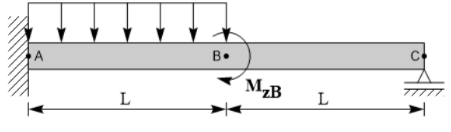
\includegraphics[width=.9\textwidth]{imgs/viga_eg.png}
                        \end{minipage}
                        &
                        \begin{minipage}{.3\textwidth}
                            Corpos sujeitos \textbf{somente a cargas transversais e/ou momentos fletores}
                        \end{minipage}
                        &
                        $\sum M_z,F_y = 0$ \\ \hline

                \end{tabular}
                \caption{Tabela de Modelos para Corpos Esbeltos}
            \end{table}

        \newpage
        \subsection{Equilíbrio Interno de Corpos}
            Para começarmos a entrar no assunto de deformação dos corpos, é primeiro necessário entender que quando há o \textbf{equilíbrio estático de um corpo}, há também um \textbf{equilíbrio entre quaisquer duas
            partes internas} do corpo, que \textbf{sofrem esforços internos}, sendo eles:
            \begin{itemize}
                \item Esforços Axial $N_x(x)$
                \item Esforço Cortante $V_y(x)$
                \item Momento Fletor $M_z(x)$
                \item Momento Torsor $M_x(x)$
            \end{itemize}

            \subsubsection{Convenção de Sinais}
                Quando estivermos lidando com a análise de esforços internos e deformações de corpos, nós iremos seguir a seguinte convenção de sinais:
                \begin{figure}[h]
                    \centering
                    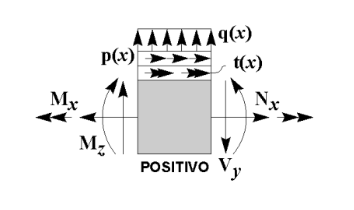
\includegraphics[width=.3\textwidth]{imgs/conv_sinais.png}
                    \caption{Convenção de Sinais para Esforços Internos}
                    \label{fig:conv_de_sinais_esf_intern}
                \end{figure}


                A partir dessa convenção e da análise dos momentos fletores $M_z$ e esforços cortantes $V_x$ conhecidos nós somos capazes de analisar a deformação de um corpo esbelto (\emph{e.g} uma viga),
                como mostrado abaixo:
                \begin{figure}[h]
                    \centering
                    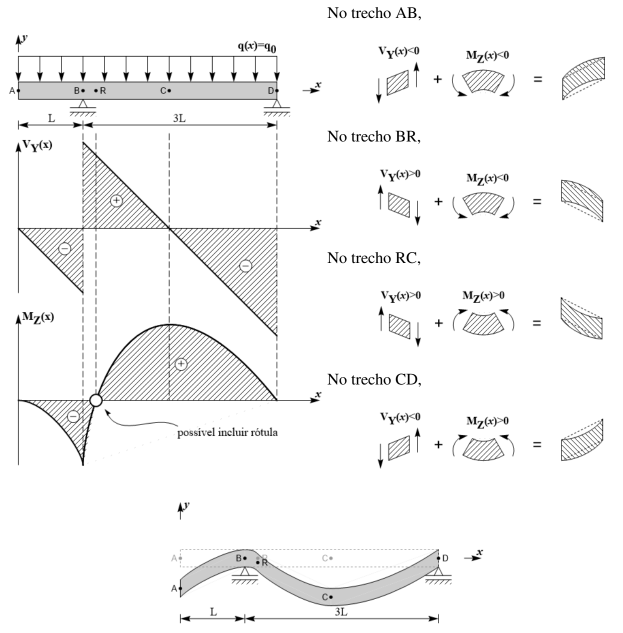
\includegraphics[width=.55\textwidth]{imgs/conv_sinais_eg.png}
                    \caption{Exemplo de Análise de Forças Internas e Deformação}
                \end{figure}

        \section{Método das Equações Diferenciais de Equilíbrio}
            \subsection{Introdução e Equações Diferenciais}
                Até o momento nós vimos que se tivermos o esforço cortante e o momento fletor para um corpo nós somos capazes de deduzir a deformação. Agora, entretanto, iremos ver como que nós calculamos
                esses valores para um corpo sofrendo carregamento. O nome do método para tal é o \textbf{Método das Equações Diferenciais}, onde nós relacionamos cada tipo de load externo (para barras,
                vigas e eixos) com as respectivas reações internas, em um cenário diferencial (para uma parte infinitesimal do corpo de cada vez, para todo o corpo), como mostrado na tabela abaixo:

                \begin{table}[h]
                    \centering
                    \begin{tabular}{|l|c|l|}\hline
                        \textbf{Cenário} & \textbf{Equação} & \textbf{Descrição}\\ \hline
                        \rule{0pt}{4ex} Barras & $\frac{d}{dx}N_x(x) = -p(x)$ & Onde $-p(x)$ é o carregamento longitudinal sendo sofrido \\[2ex]  \hline
                        \rule{0pt}{4ex} Eixos  & $\frac{d}{dx}M_x(x) = -t(x)$ & Onde $-t(x)$ é o momento axial sofrido \\[2ex]\hline
                        \rule{0pt}{4ex} Vigas: Cortante & $\frac{d}{dx}V_y(x) = +q(x)$ & Onde $+q(x)$ é o carregamento transversal sofrido \\[2ex] \hline
                        \rule{0pt}{4ex} Vigas: Momento Fletor & $\frac{d^2}{dx^2}M_z = \frac{d}{dx}V_y(x) = +q(x)$ & Onde $+q(x)$ é o carregamento transversal sofrido \\[2ex] \hline
                        
                    \end{tabular}
                    \caption{EDOs para principais modelos de corpos esbeltos}
                    \label{tb:edo_esf_internos}
                \end{table}

                Relembrando, onde:
                \begin{itemize}
                    \item Esforços Axial $N_x(x)$
                    \item Esforço Cortante $V_y(x)$
                    \item Momento Fletor $M_z(x)$
                    \item Momento Torsor $M_x(x)$
                \end{itemize}

            \newpage
            \subsection{Condições de Contorno}
                Se lembrarmos bem de calculo 3 e de equações diferenciais, todas as EDOs de grau $n$ precisam de $n$ pontos conhecidos para possam ser resolvidos, onde eles podem ser Pontos de
                Contorno ou Condições Iniciais. Para o nosso caso, iremos estudar problemas com condições de contorno.

                Para ser considerado uma condição de contorno é necessário:
                \begin{enumerate}
                    \item Estar Definida no Contorno do modelo 
                    \item Ser Conhecida a Priori
                    \item Ser Relevante para o Problema
                \end{enumerate}

                Indo além, para os nosso problemas, 99\% das vezes as condições de contorno estarão em vínculos localizados nas extremidades do corpo sendo estudado (\emph{e.g} em uma ponta de uma viga). Iremos abaixo
                \textbf{descrever as condições de contorno para os principais vínculos/apoios QUANDO PRESENTES NAS EXTREMIDADES DO CORPO}\footnote{Como estamos lidando com análise no eixo $x$, somente
                os vínculos que estão localizados nas extremidades (em $x=0$ ou $x=L$) são possíveis condições de contorno}.

                \begin{table}[h]
                    \centering
                    \begin{tabular}{|l|c|l|}\hline
                        \textbf{Vínculo} & \textbf{Equações} & \textbf{Observações} \\ \hline
                        Extremidade Livre  & 
                            \begin{minipage}{.4\textwidth}
                                \begin{align*}
                                    \sum M = 0 \\ 
                                    \sum F = 0
                                \end{align*}
                            \end{minipage} &
                            
                            \begin{minipage}{.4\textwidth}
                                \vspace{5px}
                                Como uma extremidade livre não apresenta reação a força nem momento, \textbf{se não for dito que há um valor diferente} para tais, na extremidade em questão os valores serão zero.
                            \end{minipage} \\ \hline

                        Rolete & 
                            \begin{minipage}{.4\textwidth}
                                \begin{align*}
                                    \sum M = 0
                                \end{align*}
                            \end{minipage} &
                            
                            \begin{minipage}{.4\textwidth}
                                \vspace{5px}
                                Como um rolete não apresenta reação a momento, \textbf{se não for dito que há um valor diferente}, na extremidade em questão  o momento é zero (condição de contorno).
                            \end{minipage} \\ \hline                       

                        Pino & 
                            \begin{minipage}{.4\textwidth}
                                \begin{align*}
                                    \sum M = 0
                                \end{align*}
                            \end{minipage} &
                            
                            \begin{minipage}{.4\textwidth}
                                \vspace{5px}
                                Como um rolete não apresenta reação a momento, \textbf{se não for dito que há um valor diferente}, na extremidade em questão o momento é zero (condição de contorno).
                            \end{minipage} \\ \hline    
                    \end{tabular}
                    \caption{Condições de Contorno para cada Vínculo}
                    \label{tb:cond_contorno}
                \end{table}

            \newpage
            \subsection{Função de Singularidade}
                Até o momento vimos que podemos modelar os esforços e momentos interno de um corpo por equações diferenciais (como visto na tabela \ref{tb:edo_esf_internos}), e que para resolve-las
                nós precisamos de condições de contorno (como visto na tabela \ref{tb:cond_contorno}). Antes de podermos resolver tais EDOs, entretanto, nós precisamos descrever os carregamentos
                externos que o corpo está sofrendo (que seriam os membros do lado direito das EDOs).

                Para casos em que os carregamentos são contínuos tal tarefa é extremamente fácil, só igualar a EDO ao valor (ou equação contínua) para todo $x$. Para os casos em que os carregamentos não são contínuos, entretanto, isso não é tão simples.

                Para casos onde o carregamento não é contínuo, nós usaremos uma notação que simplifica toda a matemática complexa chamada de \textbf{Função de Singularidade}, onde:

                \begin{align}
                    \langle x - a\rangle^m = \begin{cases}
                        0          & x<a \\ 
                        (x-a)^m    & x \ge a
                    \end{cases}
                    \label{eq:func_singularidade}
                \end{align}

                Onde a porção $\langle x - a \rangle$ rege a partir de qual ponto para de ser zero e o expoente $m$ rege o comportamento da curva a partir desse ponto, como mostra a figura abaixo:

                \begin{table}[h]
                    \centering
                    \begin{tabular}{|c|c|l|} \hline
                        \textbf{F. de Singularidade} & \textbf{Gráfico} & \textbf{Use Cases} \\ \hline
                        $\langle x - a\rangle^0$ & 
                            \begin{minipage}{.3\textwidth}
                                \centering
                                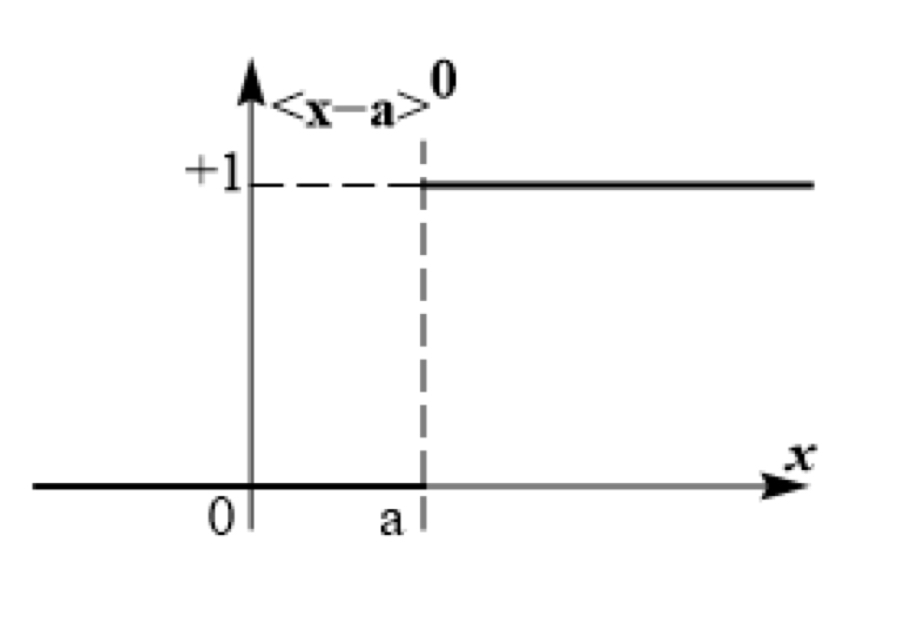
\includegraphics[width=.8\textwidth]{imgs/func_singul_0.jpeg}
                            \end{minipage}&
                            \begin{minipage}{.4\textwidth}
                                Usado mais durante análise de Vigas, quando há um carregamento de forças transversais para somente um intervalo da viga (\emph{e.g} de $L/2 \le x \le L$). Podemos,
                                ainda, subtrair dois com um shift para ter um intervalo entre $a$ e $b$, como: $\langle x - a\rangle^0 - \langle x - b\rangle^0$ 
                            \end{minipage}  \\ \hline

                        $\langle x - a\rangle^1$ & 
                            \begin{minipage}{.3\textwidth}
                                \centering
                                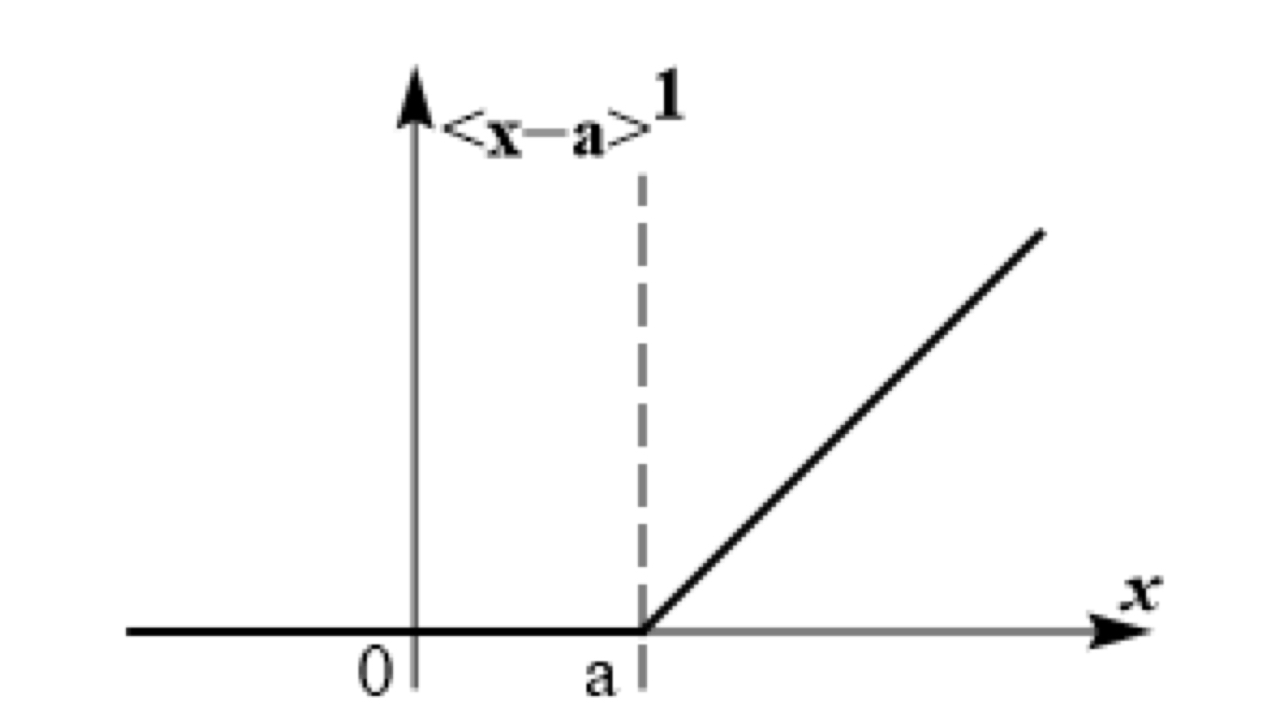
\includegraphics[width=.7\textwidth]{imgs/func_singul_1.jpeg}
                            \end{minipage}&
                            \begin{minipage}{.4\textwidth}
                                Também usado mais para análise de carregamento de vigas, mas nesse caso a força é zero até certo ponto $a$ e depois segue uma distribuição linear.
                            \end{minipage}  \\ \hline

                        $\langle x - a\rangle^2$ & 
                            \begin{minipage}{.3\textwidth}
                                \centering
                                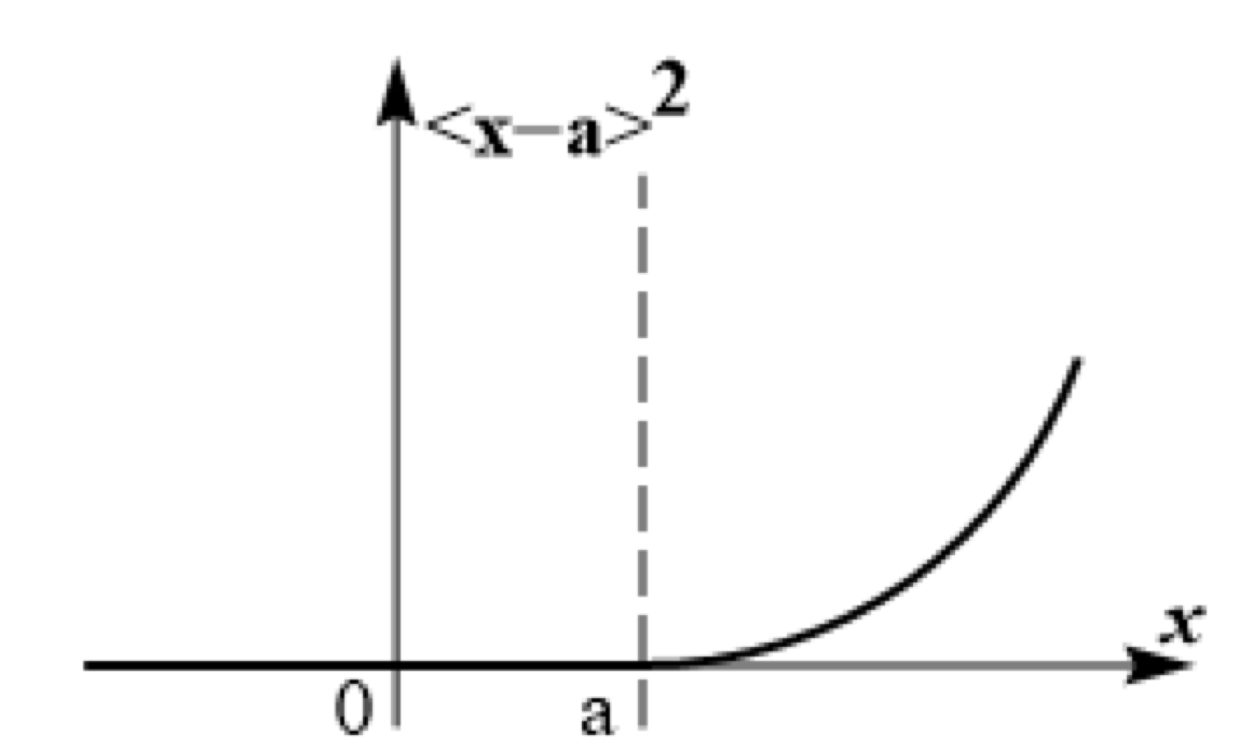
\includegraphics[width=.7\textwidth]{imgs/func_singul_2.jpeg}
                            \end{minipage}&
                            \begin{minipage}{.4\textwidth}
                                Também usado mais para análise de carregamento de vigas, mas nesse caso a força é zero até certo ponto $a$ e depois segue uma distribuição quadrática.
                            \end{minipage}  \\ \hline
                        
                        $\langle x - a\rangle^{-1}$ & 
                            \begin{minipage}{.3\textwidth}
                                \centering
                                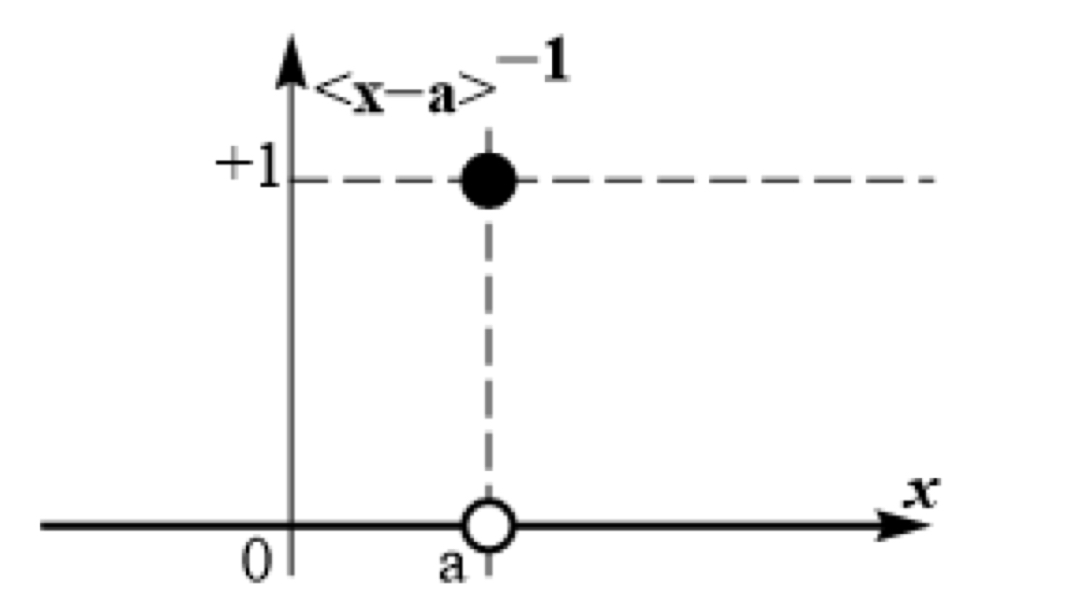
\includegraphics[width=.7\textwidth]{imgs/func_singul_-1.jpeg}
                            \end{minipage}&
                            \begin{minipage}{.4\textwidth}
                                Usando bastante para representar forças pontuais durante análise de vigas, mas também usada para representar momentos durante análise de eixos.
                            \end{minipage}  \\ \hline

                        $\langle x - a\rangle^{-2}$ & 
                            \begin{minipage}{.3\textwidth}
                                \centering
                                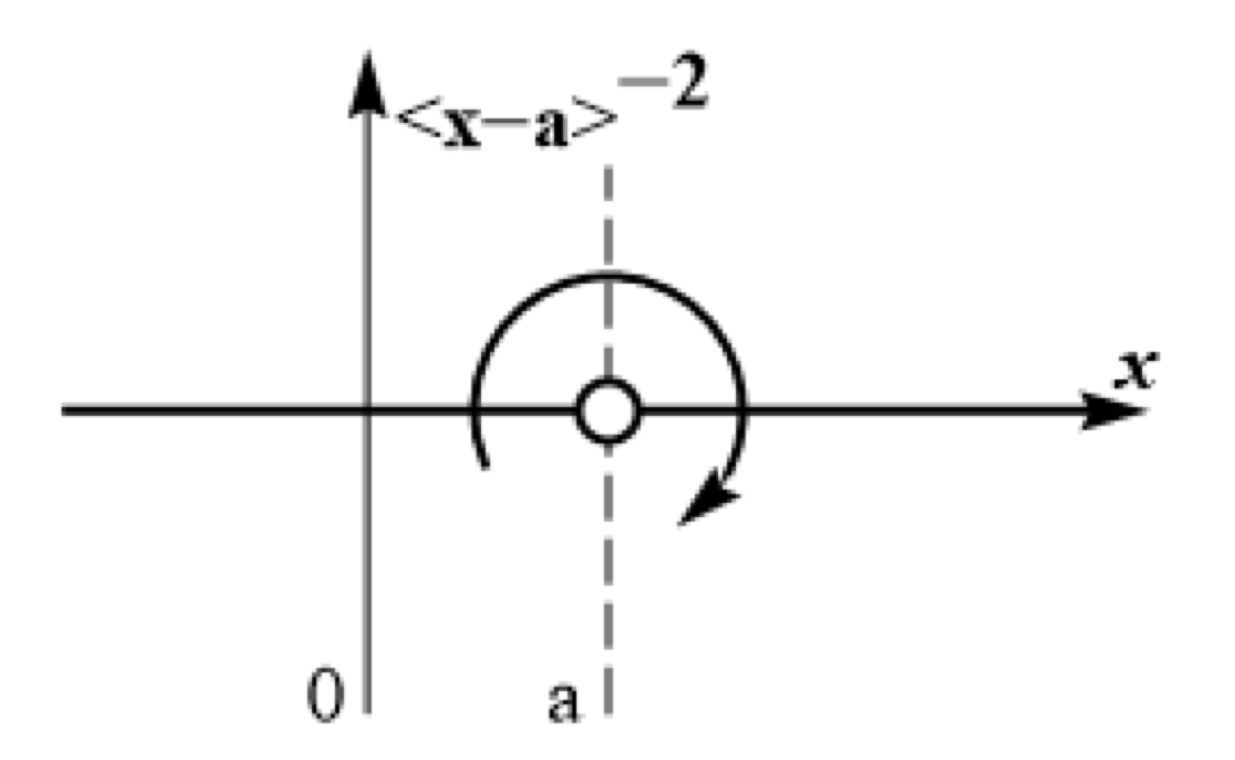
\includegraphics[width=.7\textwidth]{imgs/func_singul_-2.jpeg}
                            \end{minipage}&
                            \begin{minipage}{.4\textwidth}
                                Usado bastante durante análise de vigas para representar momentos fletores.
                            \end{minipage}  \\ \hline

                    \end{tabular}
                \end{table}

                Além disso, é importante entendermos o comportamento das funções de singularidade em relação a integração:
                \begin{align*}
                    \int \langle x-a\rangle^m dx &= \frac{\langle x - a \rangle ^{m+1}}{m + 1}, m \ge 0 \\ 
                    \int \langle x-a\rangle^{-1} dx &= \langle x - a \rangle^0 \\ 
                    \int \langle x-a\rangle^{-2} dx &= \langle x - a \rangle^{-1} \\ 
                \end{align*}

            \subsection{Método de Resolução - Equações Diferenciais de Equilíbrio}
                Já vimos quais EDOs são aplicáveis para cada modelo, os possíveis valores de contorno e também como modelar as cargas externas sendo aplicadas, o que nos resta agora é saber como
                juntar todos esses dados em um problema para resolve-lo. Para isso, nós vamos seguir 7 passos, como mostrado abaixo:
                \begin{enumerate}\addtocounter{enumi}{-1}%
                    \item Separar Carregamentos externos que são separáveis em seus respectivos modelos (barra, eixo, viga).
                    \item Estabelecer uma convenção de sinais: A fim de padronizar, seguir a convenção da figura \ref{fig:conv_de_sinais_esf_intern}
                    \item Estabelecer uma equação diferencial: A partir da tabela \ref{tb:edo_esf_internos}
                    \item Descrever condições de Contorno: Bom indicativo é começar pelos da tabela \ref{tb:cond_contorno}
                    \item Integrar a equação diferencial: Como mostrado na subsection anterior
                    \item Determinar Constantes de Integração: Substituindo os valores de contorno (já que são os únicos pontos conhecidos)
                \end{enumerate}

                Temos, ainda, algumas observações que podem ajudar a fazer os exercícios:
                \begin{itemize}
                    \item Se há uma carga distribuída que é aplicada sobre um possível ponto de contorno (\emph{e.g} como uma extremidade livre de um eixo engastado) por ela ser DISTRIBUÍDA, em um só
                    ponto ela é igual a zero logo A CONDIÇÃO DE CONTORNO AINDA É VÁLIDA. Então se for uma extremidade livre, mesmo com um momento torsor distribuído sendo aplicado, no ponto ele é zero.
                \end{itemize}

                \newpage
            \subsection{One Pager}

            Equações Diferenciais por Modelo de Corpo Esbelto:

            \begin{table}[h]\tiny
                
            \begin{tabularx}{\textwidth}{|X|X|X|}\hline
                    \textbf{Cenário} & \textbf{Equação} & \textbf{Descrição}\\ \hline
                    \rule{0pt}{4ex} Barras - Esforço Axial & $\frac{d}{dx}N_x(x) = -p(x)$ & Onde $-p(x)$ é o carregamento longitudinal sendo sofrido \\[2ex]  \hline
                    \rule{0pt}{4ex} Eixos - Momento Torsor   & $\frac{d}{dx}M_x(x) = -t(x)$ & Onde $-t(x)$ é o momento axial sofrido \\[2ex]\hline
                    \rule{0pt}{4ex} Vigaa - Esforço Cortante & $\frac{d}{dx}V_y(x) = +q(x)$ & Onde $+q(x)$ é o carregamento transversal sofrido \\[2ex] \hline
                    \rule{0pt}{4ex} Vigas - Momento Fletor & $\frac{d^2}{dx^2}M_z = \frac{d}{dx}V_y(x) = +q(x)$ & Onde $+q(x)$ é o carregamento transversal sofrido \\[2ex] \hline
            \end{tabularx}

            \end{table}
            Condição de Contorno:

            

            \begin{table}[h]
                \tiny
                \centering
            \begin{tabularx}{\textwidth}{|X|X|X|}\hline
                    \textbf{Vínculo} & \textbf{Equações} & \textbf{Observações} \\ \hline
                    Extremidade Livre  & 
                        \begin{minipage}{.3\textwidth}
                            \begin{align*}
                                \sum M = 0 \\ 
                                \sum F = 0
                            \end{align*}
                        \end{minipage} &
                        
                        \begin{minipage}{.3\textwidth}
                            \vspace{5px}
                            Como uma extremidade livre não apresenta reação a força nem momento, \textbf{se não for dito que há um valor diferente} para tais, na extremidade em questão os valores serão zero.
                        \end{minipage} \\ \hline

                    Rolete & 
                        \begin{minipage}{.3\textwidth}
                            \begin{align*}
                                \sum M = 0
                            \end{align*}
                        \end{minipage} &
                        
                        \begin{minipage}{.3\textwidth}
                            \vspace{5px}
                            Como um rolete não apresenta reação a momento, \textbf{se não for dito que há um valor diferente}, na extremidade em questão  o momento é zero (condição de contorno).
                        \end{minipage} \\ \hline                       

                    Pino & 
                        \begin{minipage}{.3\textwidth}
                            \begin{align*}
                                \sum M = 0
                            \end{align*}
                        \end{minipage} &
                        
                        \begin{minipage}{.3\textwidth}
                            \vspace{5px}
                            Como um rolete não apresenta reação a momento, \textbf{se não for dito que há um valor diferente}, na extremidade em questão o momento é zero (condição de contorno).
                        \end{minipage} \\ \hline    
                \end{tabularx}
            \end{table}

            \begin{todolist}\tiny
                \item Estar Definida no Contorno do modelo 
                \item Ser Conhecida a Priori
                \item Ser Relevante para o Problema
            \end{todolist}

            Definição de Função de Singularidade:
            \begin{table}[h]
                \tiny
                \centering
                \begin{tabularx}{\textwidth}{|X|X|l|}\hline
                    \textbf{F. de Singularidade} & \textbf{Gráfico} & \textbf{Use Cases} \\ \hline
                    $\langle x - a\rangle^0$ & 
                        \begin{minipage}{.3\textwidth}
                            \centering
                            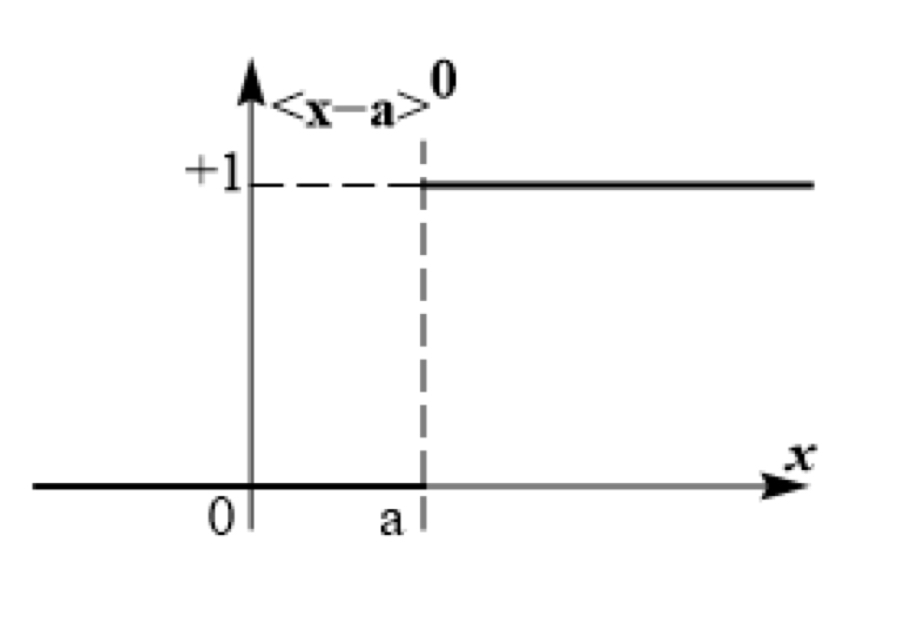
\includegraphics[width=.3\textwidth]{imgs/func_singul_0.jpeg}
                        \end{minipage}&
                        \begin{minipage}{.4\textwidth}
                            Usado mais durante análise de Vigas, quando há um carregamento de forças transversais para somente um intervalo da viga (\emph{e.g} de $L/2 \le x \le L$). Podemos,
                            ainda, subtrair dois com um shift para ter um intervalo entre $a$ e $b$, como: $\langle x - a\rangle^0 - \langle x - b\rangle^0$ 
                        \end{minipage}  \\ \hline

                    $\langle x - a\rangle^1$ & 
                        \begin{minipage}{.3\textwidth}
                            \centering
                            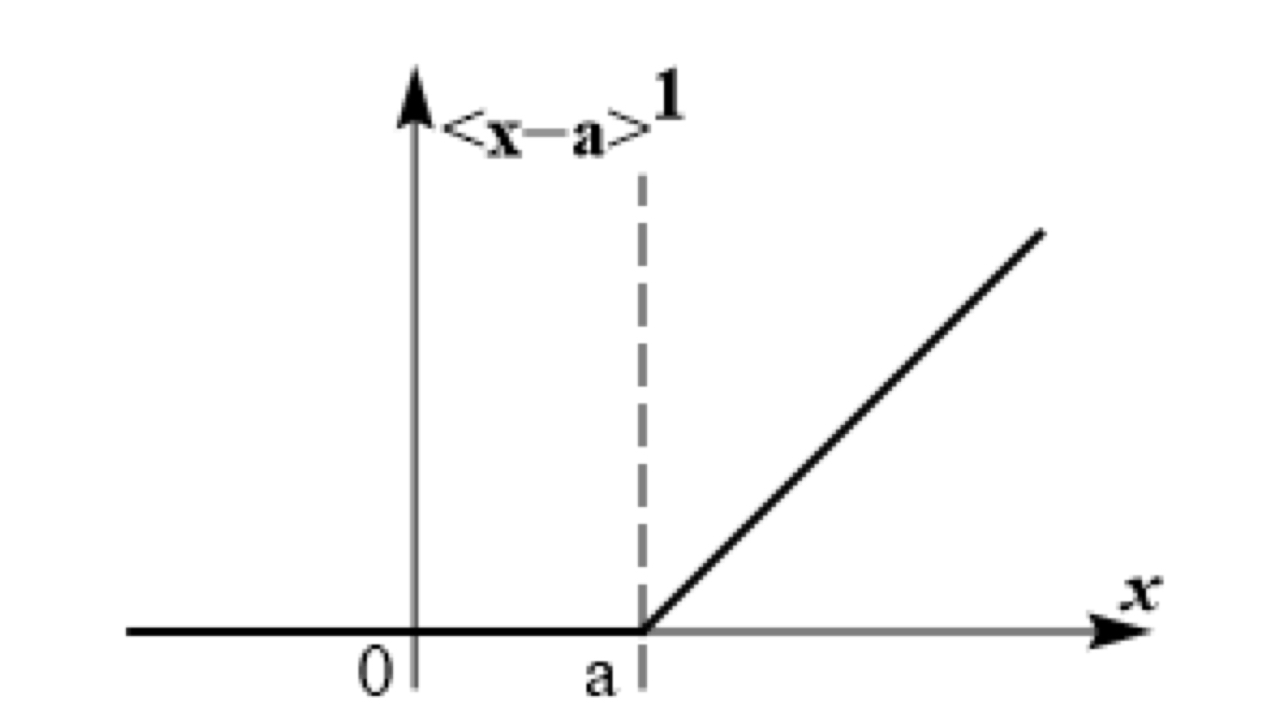
\includegraphics[width=.3\textwidth]{imgs/func_singul_1.jpeg}
                        \end{minipage}&
                        \begin{minipage}{.4\textwidth}
                            Também usado mais para análise de carregamento de vigas, mas nesse caso a força é zero até certo ponto $a$ e depois segue uma distribuição linear.
                        \end{minipage}  \\ \hline

                    $\langle x - a\rangle^2$ & 
                        \begin{minipage}{.3\textwidth}
                            \centering
                            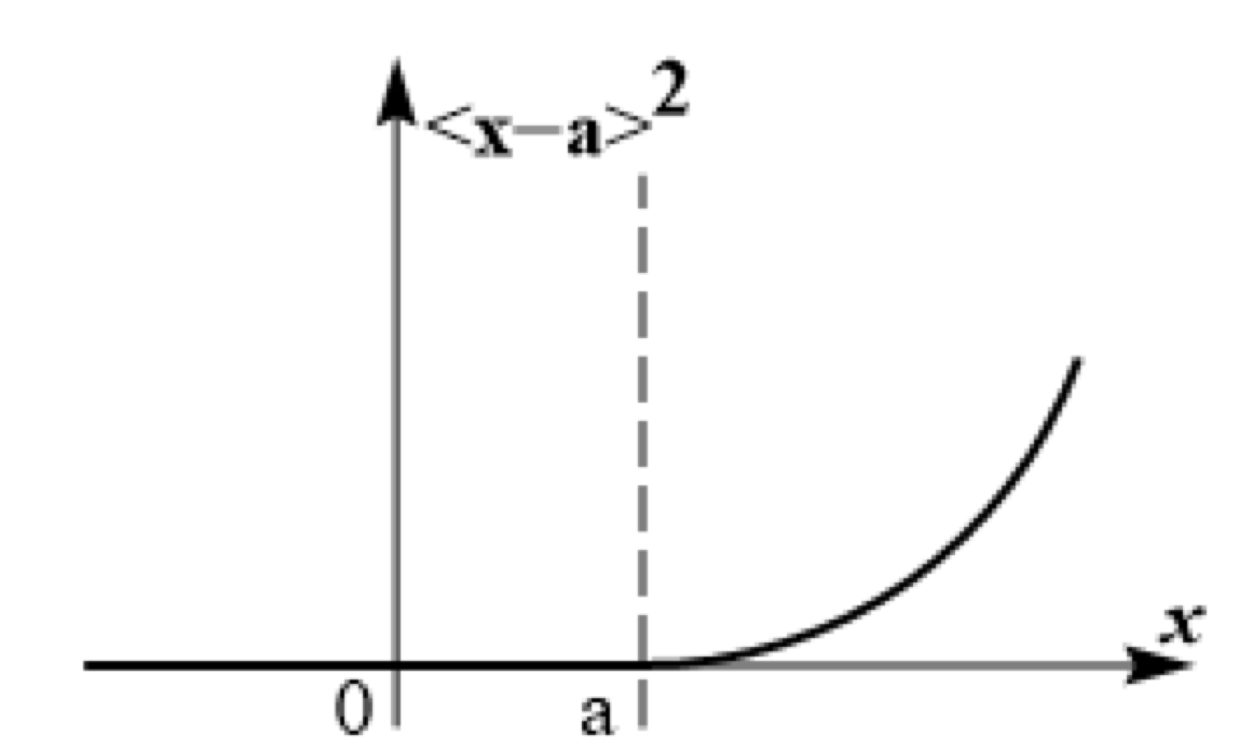
\includegraphics[width=.3\textwidth]{imgs/func_singul_2.jpeg}
                        \end{minipage}&
                        \begin{minipage}{.4\textwidth}
                            Também usado mais para análise de carregamento de vigas, mas nesse caso a força é zero até certo ponto $a$ e depois segue uma distribuição quadrática.
                        \end{minipage}  \\ \hline
                    
                    $\langle x - a\rangle^{-1}$ & 
                        \begin{minipage}{.3\textwidth}
                            \centering
                            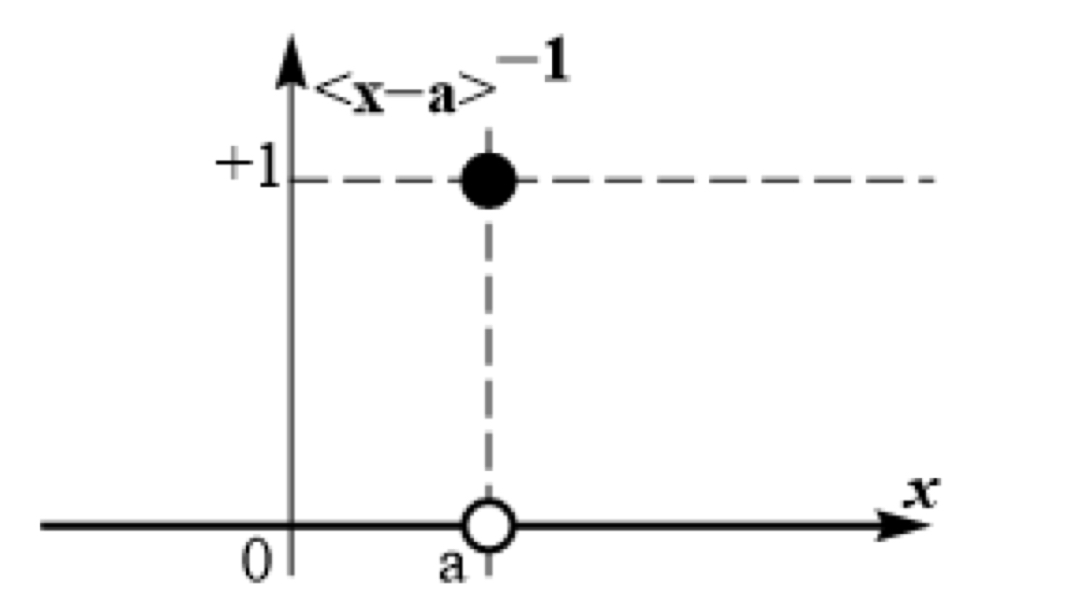
\includegraphics[width=.3\textwidth]{imgs/func_singul_-1.jpeg}
                        \end{minipage}&
                        \begin{minipage}{.4\textwidth}
                            Usando bastante para representar forças pontuais durante análise de vigas, mas também usada para representar momentos durante análise de eixos.
                        \end{minipage}  \\ \hline

                    $\langle x - a\rangle^{-2}$ & 
                        \begin{minipage}{.3\textwidth}
                            \centering
                            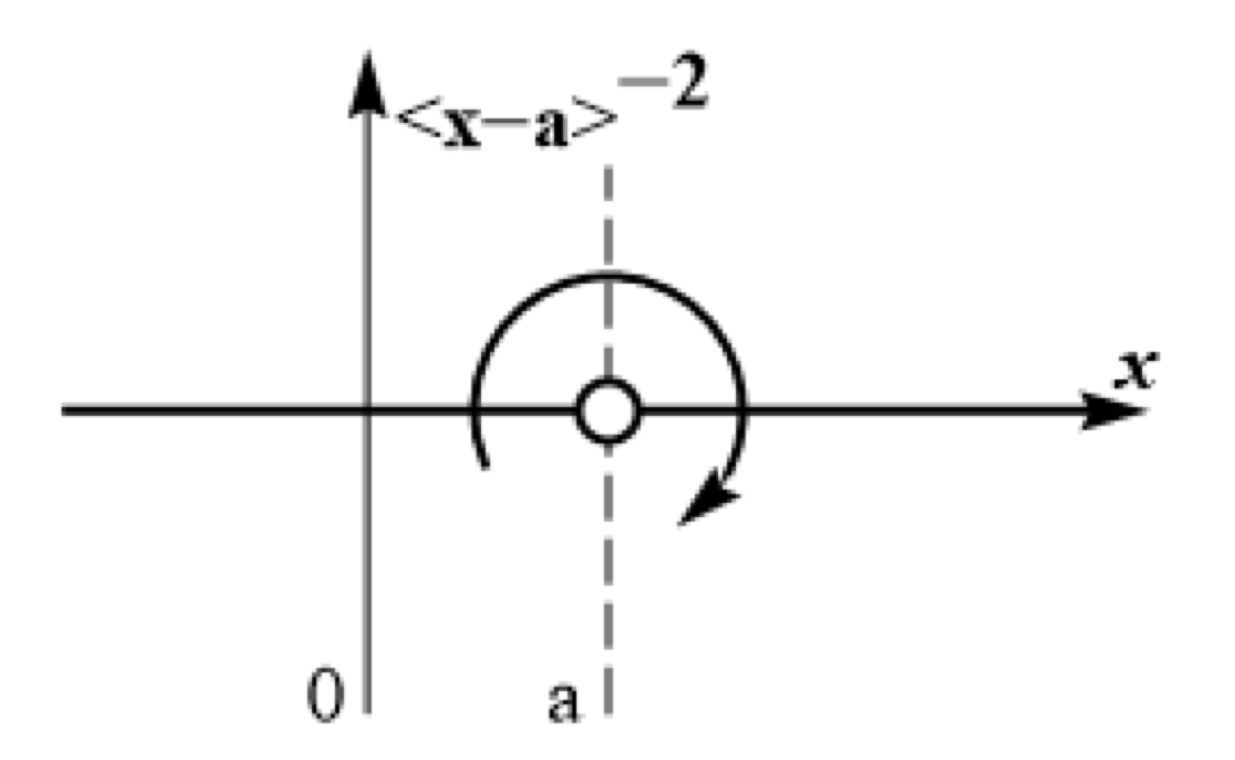
\includegraphics[width=.3\textwidth]{imgs/func_singul_-2.jpeg}
                        \end{minipage}&
                        \begin{minipage}{.4\textwidth}
                            Usado bastante durante análise de vigas para representar momentos fletores.
                        \end{minipage}  \\ \hline

                \end{tabularx}
            \end{table}

            Integração de Função de Singularidade:

            \begin{minipage}{\textwidth}\tiny
                \begin{align*}
                    \int \langle x-a\rangle^m dx &= \frac{\langle x - a \rangle ^{m+1}}{m + 1}, m \ge 0 \\ 
                    \int \langle x-a\rangle^{-1} dx &= \langle x - a \rangle^0 \\ 
                    \int \langle x-a\rangle^{-2} dx &= \langle x - a \rangle^{-1} \\ 
                \end{align*}
            \end{minipage}

            Passo a Passo:
            \begin{enumerate}\addtocounter{enumi}{-1}\tiny
                \item Separar Carregamentos externos que são separáveis em seus respectivos modelos (barra, eixo, viga).
                \item Estabelecer uma convenção de sinais: A fim de padronizar, seguir a convenção da figura \ref{fig:conv_de_sinais_esf_intern}
                \item Estabelecer uma equação diferencial: A partir da tabela \ref{tb:edo_esf_internos}
                \item Descrever condições de Contorno: Bom indicativo é começar pelos da tabela \ref{tb:cond_contorno}
                \item Integrar a equação diferencial: Como mostrado na subsection anterior
                \item Determinar Constantes de Integração: Substituindo os valores de contorno (já que são os únicos pontos conhecidos)
            \end{enumerate}




    
\end{document}